\section{Preliminaries}\label{section: preliminaries}
See \cite{kemenysnell1983} or \cite{norris1998markov}
for basic facts about Markov chains.
Throughout this paper, except where otherwise noted, 
Markov chains are assumed to have a finite state space
indexed by positive integers $1,\dots,n$ for some $n$; 
when we consider Markov chains with countably infinite state spaces, 
we will assume that for each state $i$
there are only finitely many states $j$ such that 
the transition probability $P_{ij}$ from state $i$ to state $j$ is positive.
We can represent a Markov chain by a weighted directed graph $G=(V,E)$ 
whose vertices $v_i \in V$ are the allowed states 
and the weight of the directed edge $(v_i,v_j) \in E$ is $P_{ij}$.
For brevity, we will use the words state and vertex to refer to 
both the state in the Markov chain and the corresponding vertex in $G$,
passing back and forth between the abstract Markov chain
and its concrete embodiment as a random walk on $G$.
We say that state $i$ is an \textbf{absorbing state} if $P_{ii}=1$
(equivalently if $G$ has a loop at $v_i$ with weight 1).
Notice that for every vertex $v \in G$, 
the sum of the weights of all edges $(v,w)$ is 1. 

Let $H=P-I$, where $I$ is the $n$-by-$n$ identity matrix.
Let $H_i$, $P_i$, and $I_i$ denote the $i$th rows 
of the matrices $H$, $P$, and $I$ respectively.
Observe that $I_i = e_i$ (the $i$th unit vector)
and that $-H$ is the Laplacian of the graph.
The Markov chain admits at least one \textbf{stationary measure} $\ppi$
for which the vector $v = [\ppi(1),\dots,\ppi(n)]$ satisfies $vP=v$
(this follows from the assumption that the Markov chain is finite;
see, e.g., \cite{norris1998markov}),
so 1 is an eigenvalue of $P$ and 0 is an eigenvalue of $H$.
All eigenvalues of $P$ have magnitude at most 1.
When the Markov chain is \textbf{irreducible}
(that is, when every state can be reached from every other state
in some finite number of steps), 1 is a simple eigenvalue of $P$
and 0 is a simple eigenvalue of $H$,
so that $H$ has rank $n-1$,
and the rows of $H$, taken with integer coefficients,
generate an $n-1$-dimensional sublattice of the 
space of vectors with entries summing to zero;
in this case, there is a unique stationary measure $\ppi$
satisfying $\ppi(1)+\cdots+\ppi(n) = 1$.

We now informally introduce the hunger game on the weighted directed graph $G$
by comparing it to the chip-firing model and the rotor-router model
before offering a more technical definition.

The ``goodness'' of a deterministic analogue of a random process
can be assessed by the notion of discrepancy.
If some numerical characteristic of the deterministic process
converges to a corresponding numerical characteristic of the random process
as simulation time goes to infinity,
one can try to determine the rate of convergence.

The simplest deterministic analogues of Markov chains
were invented by Engel \cite{engel1975probabilistic,engel1976does}, 
under the name \textbf{the stochastic abacus}
(though the term \textbf{chip-firing} is more common nowadays).
Suppose that all the transition probabilities $P_{ij}$ are rational,
and that we have positive integers $d_1,\dots,d_n$
such that $d_i P_{ij}$ is an integer for all $i,j$.
Assume that the Markov chain is irreducible.
Define a \textbf{chip-configuration} as 
an $n$-tuple $\mathbf{c} = (\mathbf{c}_1,\dots,\mathbf{c}_n)$;
say that a chip-configuration is \textbf{stable}
if $\mathbf{c}_i < d_i$ whenever $i$ is a non-absorbing state.
If $\mathbf{c}_i \geq d_i$, then we obtain another chip-configuration 
by \textbf{firing at $i$}, replacing $\mathbf{c}$ by
$\mathbf{c'} = \mathbf{c} + d_i H_i$;
if we represent the Markov chain by drawing a graph with vertices $v_1,\dots,v_n$
and we represent the chip-configuration $\mathbf{c}$ 
by putting $\mathbf{c}_j$ chips at $v_j$ for all $j$,
then firing means sending $d_i P_{ij}$ chips 
from $i$ to $j$ for each $j \neq i$.
% Snell \cite{snell1979}, filling in details missing from Engel's articles,
% showed how one can use chip-firing to compute the probability
% when $u$ is a nonabsorbing state and $v$ is an absorbing state,
% that a random walker started at a particular nonabsorbing state
% will eventually reach a particular absorbing state.
% In this procedure, when there are multiple non-stable states,
% one can apply firing at any one of them.
Chip-firing can be used to find the stationary probability measure 
of an irreducible Markov chain as follows.
Put sufficiently many chips on the state-graph so that 
stabilization is impossible no matter how many firings are performed, 
and start performing firings however one wishes;
when we encounter a chip-configuration we have seen before
(as must happen eventually), the vector that records the number of times
each state has fired will be a stationary vector.

\begin{example}\label{example: 3 chip}
Suppose we have the Markov chain given by the Markov matrix
\begin{align*}
    \begin{bmatrix}
        \frac{1}{2} & \frac{1}{2} & 0 \\
        \frac{1}{2} & 0 & \frac{1}{2} \\
        0 & \frac{1}{2} & \frac{1}{2}
    \end{bmatrix},
\end{align*}
representing a doubly-reflecting random walk.
Its corresponding graph is shown in \cref{fig:ex2G}\,.
\begin{figure}[htbp]
    \centering
    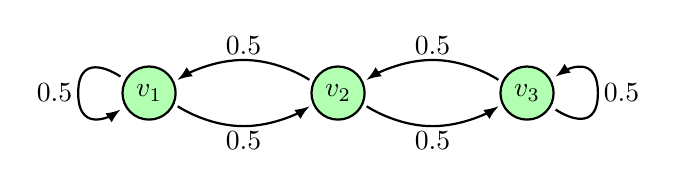
\begin{tikzpicture}[scale=0.6,font=\normalsize,baseline,thick]
        \foreach \x in {1,...,3} {
            \filldraw[color=black,fill=green!30,thick] (4*\x,0) circle (16pt);
            \node at (4*\x,0) {$v_{\x}$};
        }
        % Left arrows
        \foreach \x in {2,3} {
            \draw [->,>=latex] plot [smooth,tension=1] coordinates {(4*\x-0.866*0.7,0.4*0.7) (4*\x-2,0.7) (4*\x-4+0.866*0.7,0.4*0.7)};
        }
        % Right arrows
        \foreach \x in {1,2} {
            \draw [->,>=latex] plot [smooth,tension=1] coordinates {(4*\x+0.866*0.7,-0.4*0.7) (4*\x+2,-0.7) (4*\x+4-0.866*0.7,-0.4*0.7)};
        }
        \node at (6,1) {0.5};
        \node at (10,1) {0.5};
        \node at (6,-1) {0.5};
        \node at (10,-1) {0.5};
        \draw [->,>=latex] plot [smooth,tension=5] coordinates {(4-0.866*0.7,0.5*0.7) (4-1.5,0) (4-0.866*0.7,-0.5*0.7)};
        \node at (2,0) {0.5};
        \draw [->,>=latex] plot [smooth,tension=5] coordinates {(12+0.866*0.7,-0.5*0.7) (12+1.5,0) (12+0.866*0.7,0.5*0.7)};
        \node at (14,0) {0.5};
    \end{tikzpicture}
    \caption{A graph $G$ corresponding to a doubly-reflecting random walk.}
    \label{fig:ex2G}
\end{figure}
If we place 1 chip at state 1, 2 chips at state 2, and 1 chip at state 3,
then state 2 is unstable, so we may fire at 2,
turning the chip-configuration (1,2,1) into the chip-configuration (2,0,2).
Then firing at 1 and at 3 brings us back to (1,2,1).
The vector that records the number of times each state fired
is (1,1,1), which is indeed a stationary vector for this Markov chain.
\end{example}

The rotor-router model~\cite{holroyd2010rotor}
is a different scheme for imitating Markov chains deterministically.
Assume as above that the Markov chain
has rational transition probabilities, with $d_i$ as above.
Represent the Markov chain using a directed graph
with $d_i P_{ij}$ parallel edges from $v_i$ to $v_j$,
so that $v_i$ has outdegree $d_i$.
Each vertex distributes arriving chips along its outgoing edges in a cyclic manner, 
not sending a chip along any edge for a second time
until it has sent a chip along every edge at least once,
and thereafter always sending the next chip along 
the edge along which it has sent a chip least recently.
Inasmuch as the vertex with the chip gets to decide where the chip goes next,
we call this ``supply-side'' management of the chip's movement.
Assume that the Markov chain is irreducible.
It can be shown that once the chip enters an infinite loop
(as must happen eventually),
the fraction of the time that the chip spends at vertex $v_i$
is proportional to the steady-state $\ppi(i)$.

\begin{example}\label{example: 3 rotor}
We use the same Markov chain as~\cref{example: 3 chip}.
Suppose we start with the chip at $v_1$
and begin the game by sending the chip to $v_2$, then $v_3$, then $v_3$ again.
Since at this point the chip has already traveled 
along the edge sending $v_3$ to $v_3$,
it now travels along the edge from $v_3$ to $v_2$.
As the chip has already gone from $v_2$ to $v_3$,
the rotor-router protocol dictates
that it must now travel along the other edge from $v_2$ and go to $v_1$.
Similarly, as it has already gone from $v_1$ to $v_2$,
now it must travel from $v_1$ to $v_1$.
Thereafter the process cycles forever.
Since within each cycle
the chip spends 2 steps at each vertex,
(2,2,2) is a stationary vector.
\end{example}

The \textbf{hunger game} introduced in this article
can be seen as a ``demand-side" management system: 
each vertex has a ``hunger" for chips, 
determined by its expectation of receiving chips 
from neighboring vertices that have been previously visited.
When a vertex $v$ receives a chip, the neighboring vertices' hunger 
increases in accordance to the transition probabilities from $v$ 
to those vertices, and $v$ sends its chip to the vertex with highest hunger
(regardless of whether that chip is a neighbor of $v$).

Now we give a more formal definition of the \textbf{hunger game}.
It is simplest to start with the situation
in which the chain runs forever without restarts
(in contrast to chains that will be restarted 
when they enter an absorbing state).
We also start with the case in which the state space is finite,
with $|V| = n$, deferring discussion of infinite-state spaces until later.
The \textbf{hunger vector} $\mathbf{h}\in\R^{n}$ represents 
the hunger at each vertex in $V$;
we will sometimes call it the \textbf{hunger state} to emphasize 
its interpretation as a state of the hunger game system.
At each step, whichever vertex has the highest hunger receives the chip; 
if vertex $v_i$ receives the chip, then the hunger vector $\mathbf{h}$ 
is updated by adding $H_i = P_i - I_i$ to it, corresponding to 
the increase in vertices' hunger from the presence of this chip at $v_i$ 
but also the satiation of $v_i$ after receiving a chip.
If multiple states are tied for the highest hunger,
we break the tie by choosing the lowest-indexed such vertex.
Since each row of $H$ has entries summing to 0,
total hunger never changes.

Each relocation of the chip is referred to as \textbf{firing} the chip;
specifically, when the chip is relocated at $i$,
we say the chip fires to $i$.
Unlike rotor-router or chip-firing, 
under the hunger game rules a chip does not necessarily have to be fired 
to a vertex adjacent to its current location; see \cref{example: 3 hunger}\,.
In fact, the determination of the chip's next location depends 
only on the hunger state $\mathbf{h}$ and not the current location of the chip.
The step can be described purely in terms of
the matrix $H$ and the vector $\mathbf{h}$
without any reference to chips, via the rule
``Replace $\mathbf{h}$ by $\mathbf{h}' = \mathbf{h} + H_i$
where $i$ maximizes $\mathbf{h}_i$,
choosing the smallest such $i$ in the event of a tie.'' 

\begin{example}\label{example: 3 hunger}
We use the same Markov chain as~\cref{example: 3 chip}.
Starting with $\mathbf{h}=0$, as shown in \cref{subfig:ex2init}\,, 
regardless of the initial location of the chip, we fire the chip to $v_1$ 
under the tie-breaking rule, 
yielding $\mathbf{h}=\left[-\frac{1}{2},\frac{1}{2},0\right]$ 
as shown in \cref{subfig:ex2fire1}\,.
After this, we fire to $v_2$, as shown in \cref{subfig:ex2fire2}\,, 
and then fire to $v_3$, as shown in \cref{subfig:ex2fire3}\,.
Notice that we have returned back to 
the initial hunger state $\mathbf{h}=\mathbf{0}$, 
so this process repeats, 
visiting states 1, 2, 3, then back to 1, and so on.
Notice that we fire the chip from 3 to 1
even though $P_{31}=0$.
\begin{figure}[htbp]
    \centering
    \begin{subfigure}{\textwidth}
        \centering
        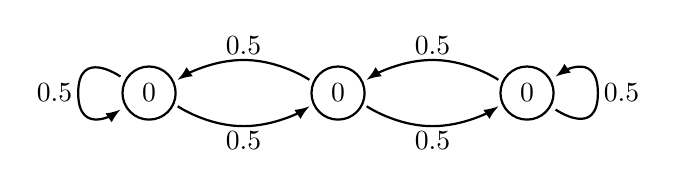
\begin{tikzpicture}[scale=0.6,font=\normalsize,baseline,thick]
            \foreach \x/\xcolor in {1/white,2/white,3/white} {
                \filldraw[color=black,fill=\xcolor,thick] (4*\x,0) circle (16pt);
            }
            \foreach \x/\xtext in {1/0,2/0,3/0} {
                \node at (4*\x,0) {\xtext};
            }
            % Left arrows
            \foreach \x in {2,3} {
                \draw [->,>=latex] plot [smooth,tension=1] coordinates {(4*\x-0.866*0.7,0.4*0.7) (4*\x-2,0.7) (4*\x-4+0.866*0.7,0.4*0.7)};
            }
            % Right arrows
            \foreach \x in {1,2} {
                \draw [->,>=latex] plot [smooth,tension=1] coordinates {(4*\x+0.866*0.7,-0.4*0.7) (4*\x+2,-0.7) (4*\x+4-0.866*0.7,-0.4*0.7)};
            }
            \node at (6,1) {0.5};
            \node at (10,1) {0.5};
            \node at (6,-1) {0.5};
            \node at (10,-1) {0.5};
            \draw [->,>=latex] plot [smooth,tension=5] coordinates {(4-0.866*0.7,0.5*0.7) (4-1.5,0) (4-0.866*0.7,-0.5*0.7)};
            \node at (2,0) {0.5};
            \draw [->,>=latex] plot [smooth,tension=5] coordinates {(12+0.866*0.7,-0.5*0.7) (12+1.5,0) (12+0.866*0.7,0.5*0.7)};
            \node at (14,0) {0.5};
        \end{tikzpicture}
        \caption{The initial hunger state $\mathbf{h}=\mathbf{0}$.}
        \label{subfig:ex2init}
    \end{subfigure}
    \begin{subfigure}{\textwidth}
        \centering
        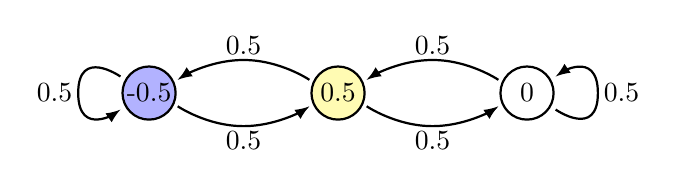
\begin{tikzpicture}[scale=0.6,font=\normalsize,baseline,thick]
            \foreach \x/\xcolor in {1/blue!30,2/yellow!30,3/white} {
                \filldraw[color=black,fill=\xcolor,thick] (4*\x,0) circle (16pt);
            }
            \foreach \x/\xtext in {1/-0.5,2/0.5,3/0} {
                \node at (4*\x,0) {\xtext};
            }
            % Left arrows
            \foreach \x in {2,3} {
                \draw [->,>=latex] plot [smooth,tension=1] coordinates {(4*\x-0.866*0.7,0.4*0.7) (4*\x-2,0.7) (4*\x-4+0.866*0.7,0.4*0.7)};
            }
            % Right arrows
            \foreach \x in {1,2} {
                \draw [->,>=latex] plot [smooth,tension=1] coordinates {(4*\x+0.866*0.7,-0.4*0.7) (4*\x+2,-0.7) (4*\x+4-0.866*0.7,-0.4*0.7)};
            }
            \node at (6,1) {0.5};
            \node at (10,1) {0.5};
            \node at (6,-1) {0.5};
            \node at (10,-1) {0.5};
            \draw [->,>=latex] plot [smooth,tension=5] coordinates {(4-0.866*0.7,0.5*0.7) (4-1.5,0) (4-0.866*0.7,-0.5*0.7)};
            \node at (2,0) {0.5};
            \draw [->,>=latex] plot [smooth,tension=5] coordinates {(12+0.866*0.7,-0.5*0.7) (12+1.5,0) (12+0.866*0.7,0.5*0.7)};
            \node at (14,0) {0.5};
        \end{tikzpicture}
        \caption{$\mathbf{h}$ after firing to $v_1$, shown in blue. States with updated hungers are shown in yellow.}
        \label{subfig:ex2fire1}
    \end{subfigure}
    \begin{subfigure}{\textwidth}
        \centering
        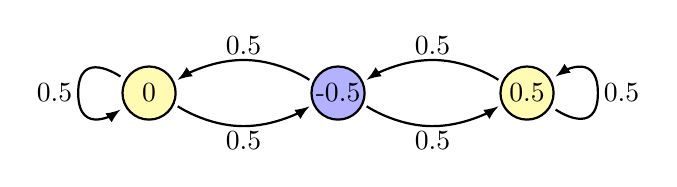
\begin{tikzpicture}[scale=0.6,font=\normalsize,baseline,thick]
            \foreach \x/\xcolor in {1/yellow!30,2/blue!30,3/yellow!30} {
                \filldraw[color=black,fill=\xcolor,thick] (4*\x,0) circle (16pt);
            }
            \foreach \x/\xtext in {1/0,2/-0.5,3/0.5} {
                \node at (4*\x,0) {\xtext};
            }
            % Left arrows
            \foreach \x in {2,3} {
                \draw [->,>=latex] plot [smooth,tension=1] coordinates {(4*\x-0.866*0.7,0.4*0.7) (4*\x-2,0.7) (4*\x-4+0.866*0.7,0.4*0.7)};
            }
            % Right arrows
            \foreach \x in {1,2} {
                \draw [->,>=latex] plot [smooth,tension=1] coordinates {(4*\x+0.866*0.7,-0.4*0.7) (4*\x+2,-0.7) (4*\x+4-0.866*0.7,-0.4*0.7)};
            }
            \node at (6,1) {0.5};
            \node at (10,1) {0.5};
            \node at (6,-1) {0.5};
            \node at (10,-1) {0.5};
            \draw [->,>=latex] plot [smooth,tension=5] coordinates {(4-0.866*0.7,0.5*0.7) (4-1.5,0) (4-0.866*0.7,-0.5*0.7)};
            \node at (2,0) {0.5};
            \draw [->,>=latex] plot [smooth,tension=5] coordinates {(12+0.866*0.7,-0.5*0.7) (12+1.5,0) (12+0.866*0.7,0.5*0.7)};
            \node at (14,0) {0.5};
        \end{tikzpicture}
        \caption{$\mathbf{h}$ after firing to $v_2$, shown in blue. States with updated hungers are shown in yellow.}
        \label{subfig:ex2fire2}
    \end{subfigure}
    \begin{subfigure}{\textwidth}
        \centering
        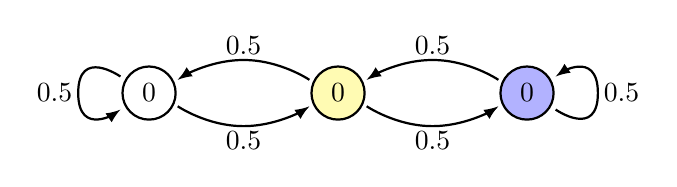
\begin{tikzpicture}[scale=0.6,font=\normalsize,baseline,thick]
            \foreach \x/\xcolor in {1/white,2/yellow!30,3/blue!30} {
                \filldraw[color=black,fill=\xcolor,thick] (4*\x,0) circle (16pt);
            }
            \foreach \x/\xtext in {1/0,2/0,3/0} {
                \node at (4*\x,0) {\xtext};
            }
            % Left arrows
            \foreach \x in {2,3} {
                \draw [->,>=latex] plot [smooth,tension=1] coordinates {(4*\x-0.866*0.7,0.4*0.7) (4*\x-2,0.7) (4*\x-4+0.866*0.7,0.4*0.7)};
            }
            % Right arrows
            \foreach \x in {1,2} {
                \draw [->,>=latex] plot [smooth,tension=1] coordinates {(4*\x+0.866*0.7,-0.4*0.7) (4*\x+2,-0.7) (4*\x+4-0.866*0.7,-0.4*0.7)};
            }
            \node at (6,1) {0.5};
            \node at (10,1) {0.5};
            \node at (6,-1) {0.5};
            \node at (10,-1) {0.5};
            \draw [->,>=latex] plot [smooth,tension=5] coordinates {(4-0.866*0.7,0.5*0.7) (4-1.5,0) (4-0.866*0.7,-0.5*0.7)};
            \node at (2,0) {0.5};
            \draw [->,>=latex] plot [smooth,tension=5] coordinates {(12+0.866*0.7,-0.5*0.7) (12+1.5,0) (12+0.866*0.7,0.5*0.7)};
            \node at (14,0) {0.5};
        \end{tikzpicture}
        \caption{$\mathbf{h}$ after firing to $v_3$, shown in blue. States with updated hungers are shown in yellow.}
        \label{subfig:ex2fire3}
    \end{subfigure}
    \caption{The hunger game on a doubly-reflecting random walk.}
    \label{fig:ex2H}
\end{figure}
% In the greedy chip-firing version of the game, 
% we place two chips at each vertex in the graph.
% We fire 1, then fire 2, then fire 3,
% and are back at the original chip-configuration.
\end{example}

If one ignores the chip and focuses on the entries of the hunger vector,
the hunger game can be viewed as a greedy variant of chip-firing.
Specifically, if all entries of $\mathbf{h}$ and $P$ are rational,
we can without loss of generality assume they are all non-negative integers
(since the firing rule is invariant under affine transformation
of the hunger vector) and create a chip-configuration of the customary kind
in which the number of chips at $i$ is $\mathbf{h}_i$. 
Then the firing rule, translated to the new context,
tells us to fire the vertex $i$ that has the most chips,
with ties resolved as before.

When the state space is (countably) infinite, our hunger vectors
are infinite sequences.
We restrict ourselves to sequences that are bounded
and take on only finitely many distinct values;
this ensures that there exists at least one $i$
for which $\mathbf{h}_i$ equals $\sup_i \mathbf{h}_i$,
from which it follows that a smallest such $i$ exists.
As each vertex has only finitely many outgoing edges, 
this assumption ensures that after 
any finite number of steps in the hunger game 
there are only finitely many distinct values of hunger, 
so a vertex of highest hunger can be found
and the lowest-indexed one can be chosen, ad infinitum.

% \Rupert{Absorbing version of hunger game.}
For Markov chains with absorbing states we vary the procedure slightly.
We start with a graph devoid of chips, add a chip at an initial vertex,
and then follow the rule for moving the chip described above,
with the extra stipulation that when the chip reaches 
an absorbing vertex, it gets removed from the graph.
In more detail, we define chip addition operators $E_i$ as follows:
Given an initial hunger vector $\mathbf{h}$, 
we place a chip at $v_i$ (increasing the hunger of the neighbors of $v_i$)
and add $P_i$ to $\mathbf{h}$,
and we then repeatedly move the chip to the currently hungriest vertex
(the lowest-indexed one, in the event of a tie),
simultaneously incrementing the hunger vector
by the row of $H$ corresponding to the chip's new location,
until we arrive at an absorbing vertex $v_k$,
at which point we subtract $P_k=I_k$ from the current hunger vector
and remove the chip from $v_k$.
We define $E_i(\mathbf{h})$ to be the final hunger vector,
and call $E_i$ the \textbf{chip addition operator} at $i$.
It is possible for $E_i(\mathbf{h})$ to be undefined,
in the event that the process never arrives at an absorbing state,
but we will show in \cref{lemma: finite terminate} 
that for finite absorbing chains 
the process must terminate so that $E_i$ is well-defined;
moreover, each chip addition operator preserves total hunger,
since the sum of the entries increases by 1 when $P_i$ is added,
stays the same each time a row of $H$ is added,
and decreases by 1 when $P_k$ is subtracted.

As in the previous situation, the process can be described
purely in terms of vector and matrix operations
without reference to $G$ or a chip.
Given a vector $\mathbf{h}\in\R^{n}$, add row $P_i$ to $\mathbf{h}$.
Thereafter, if $j$ is the unique value such that 
$h_{j'} < h_j$ for all $j' < j$ and $h_j \geq h_{j'}$ for all ${j'} > j$, 
add $H_j$ to $\mathbf{h}$,
% Is this next remark needed?
% $H_{kk} \leq 0$,
% thus (weakly) decreasing $\mathbf{h}_i$, the maximum value in $\mathbf{h}$.
unless $j$ is an absorbing state (call it $k$), in which case
subtract $P_k$ from the hunger vector and stop, 
calling the result $E_i(\mathbf{h})$.

\begin{example}\label{example: absorbing 5 walk}
Suppose we have the Markov chain represented by the graph in \cref{fig:ex1G}\,.
It has absorbing states $v_1$ and $v_5$.
\begin{figure}[htbp]
    \centering
    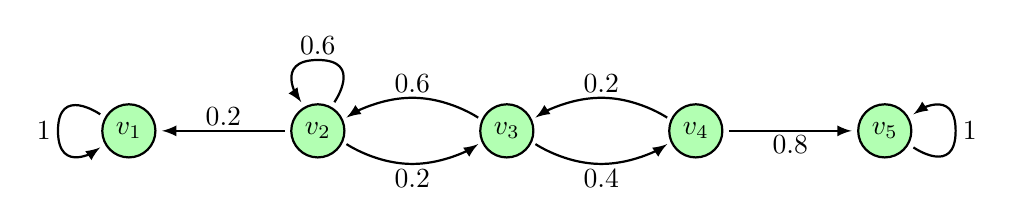
\begin{tikzpicture}[scale=0.6,font=\normalsize,baseline,thick]
        \foreach \x in {1,...,5} {
            \filldraw[color=black,fill=green!30,thick] (4*\x,0) circle (16pt);
            \node at (4*\x,0) {$v_{\x}$};
        }
        \draw [->,>=latex] plot [smooth,tension=5] coordinates {(8+0.5*0.7,0.866*0.7) (8+0,1.5) (8-0.5*0.7,0.866*0.7)};
        \node at (8,1.8) {0.6};
        \foreach \x in {3,...,4} {
            \draw [->,>=latex] plot [smooth,tension=1] coordinates {(4*\x-0.866*0.7,0.4*0.7) (4*\x-2,0.7) (4*\x-4+0.866*0.7,0.4*0.7)};
        }
        \foreach \x in {2,...,3} {
            \draw [->,>=latex] plot [smooth,tension=1] coordinates {(4*\x+0.866*0.7,-0.4*0.7) (4*\x+2,-0.7) (4*\x+4-0.866*0.7,-0.4*0.7)};
        }
        \draw[->,>=latex] (8-0.7,0) -- (4+0.7,0);
        \draw[->,>=latex] (16+0.7,0) -- (20-0.7,0);
        \node at (6,0.3) {0.2};
        \node at (10,1) {0.6};
        \node at (14,1) {0.2};
        \node at (10,-1) {0.2};
        \node at (14,-1) {0.4};
        \node at (18,-0.3) {0.8};
        \draw [->,>=latex] plot [smooth,tension=5] coordinates {(4-0.866*0.7,0.5*0.7) (4-1.5,0) (4-0.866*0.7,-0.5*0.7)};
        \node at (2.2,0) {1};
        \draw [->,>=latex] plot [smooth,tension=5] coordinates {(20+0.866*0.7,-0.5*0.7) (20+1.5,0) (20+0.866*0.7,0.5*0.7)};
        \node at (21.8,0) {1};
    \end{tikzpicture}
    \caption{A graph $G$ corresponding to an absorbing Markov chain.}
    \label{fig:ex1G}
\end{figure}
Let us compute $E_3(\mathbf{0})$.
Starting with $\mathbf{h}=\mathbf{0}$,
for our first step we add a chip to $v_3$ to yield $\mathbf{h}=[0,0.6,0,0.4,0]$,
as shown in \cref{subfig:ex1insert}\,.
After this, we follow additional steps of the hunger game process, 
firing the chip successively to $v_2$, $v_4$, and $v_5$, 
as shown in \cref{subfig:ex1fire3}\,.
Having reached an absorbing state, the final step is 
to remove the chip from $v_5$, 
resulting in $E_3(\mathbf{0})=[0.2,0.2,0.4,-0.6,-0.2]$,
as shown in \cref{subfig:ex1remove}\,.
\begin{figure}[htbp]
    \centering
    \begin{subfigure}{\textwidth}
        \centering
        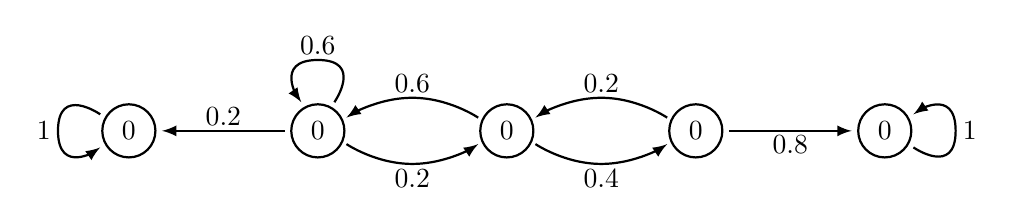
\begin{tikzpicture}[scale=0.6,font=\normalsize,baseline,thick]
            \foreach \x/\xcolor in {1/white,2/white,3/white,4/white,5/white} {
                \filldraw[color=black,fill=\xcolor,thick] (4*\x,0) circle (16pt);
            }
            \foreach \x/\xtext in {1/0,2/0,3/0,4/0,5/0} {
                \node at (4*\x,0) {\xtext};
            }
            \draw [->,>=latex] plot [smooth,tension=5] coordinates {(8+0.5*0.7,0.866*0.7) (8+0,1.5) (8-0.5*0.7,0.866*0.7)};
            \node at (8,1.8) {0.6};
            \foreach \x in {3,...,4} {
                \draw [->,>=latex] plot [smooth,tension=1] coordinates {(4*\x-0.866*0.7,0.4*0.7) (4*\x-2,0.7) (4*\x-4+0.866*0.7,0.4*0.7)};
            }
            \foreach \x in {2,...,3} {
                \draw [->,>=latex] plot [smooth,tension=1] coordinates {(4*\x+0.866*0.7,-0.4*0.7) (4*\x+2,-0.7) (4*\x+4-0.866*0.7,-0.4*0.7)};
            }
            \draw[->,>=latex] (8-0.7,0) -- (4+0.7,0);
            \draw[->,>=latex] (16+0.7,0) -- (20-0.7,0);
            \node at (6,0.3) {0.2};
            \node at (10,1) {0.6};
            \node at (14,1) {0.2};
            \node at (10,-1) {0.2};
            \node at (14,-1) {0.4};
            \node at (18,-0.3) {0.8};
            \draw [->,>=latex] plot [smooth,tension=5] coordinates {(4-0.866*0.7,0.5*0.7) (4-1.5,0) (4-0.866*0.7,-0.5*0.7)};
            \node at (2.2,0) {1};
            \draw [->,>=latex] plot [smooth,tension=5] coordinates {(20+0.866*0.7,-0.5*0.7) (20+1.5,0) (20+0.866*0.7,0.5*0.7)};
            \node at (21.8,0) {1};
        \end{tikzpicture}
        % \caption{The initial hunger state $\mathbf{h}=\mathbf{0}$.}
        % \label{subfig:before}
    \end{subfigure}
    
    \vspace{-0.5mm}
    
    \begin{subfigure}{\textwidth}
        \centering
        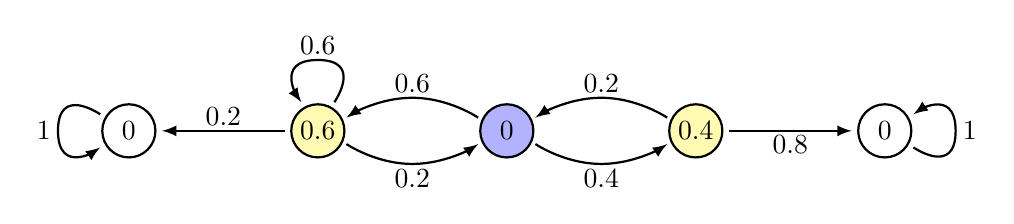
\begin{tikzpicture}[scale=0.6,font=\normalsize,baseline,thick]
            \foreach \x/\xcolor in {1/white,2/yellow!30,3/blue!30,4/yellow!30,5/white} {
                \filldraw[color=black,fill=\xcolor,thick] (4*\x,0) circle (16pt);
            }
            \foreach \x/\xtext in {1/0,2/0.6,3/0,4/0.4,5/0} {
                \node at (4*\x,0) {\xtext};
            }
            \draw [->,>=latex] plot [smooth,tension=5] coordinates {(8+0.5*0.7,0.866*0.7) (8+0,1.5) (8-0.5*0.7,0.866*0.7)};
            \node at (8,1.8) {0.6};
            \foreach \x in {3,...,4} {
                \draw [->,>=latex] plot [smooth,tension=1] coordinates {(4*\x-0.866*0.7,0.4*0.7) (4*\x-2,0.7) (4*\x-4+0.866*0.7,0.4*0.7)};
            }
            \foreach \x in {2,...,3} {
                \draw [->,>=latex] plot [smooth,tension=1] coordinates {(4*\x+0.866*0.7,-0.4*0.7) (4*\x+2,-0.7) (4*\x+4-0.866*0.7,-0.4*0.7)};
            }
            \draw[->,>=latex] (8-0.7,0) -- (4+0.7,0);
            \draw[->,>=latex] (16+0.7,0) -- (20-0.7,0);
            \node at (6,0.3) {0.2};
            \node at (10,1) {0.6};
            \node at (14,1) {0.2};
            \node at (10,-1) {0.2};
            \node at (14,-1) {0.4};
            \node at (18,-0.3) {0.8};
            \draw [->,>=latex] plot [smooth,tension=5] coordinates {(4-0.866*0.7,0.5*0.7) (4-1.5,0) (4-0.866*0.7,-0.5*0.7)};
            \node at (2.2,0) {1};
            \draw [->,>=latex] plot [smooth,tension=5] coordinates {(20+0.866*0.7,-0.5*0.7) (20+1.5,0) (20+0.866*0.7,0.5*0.7)};
            \node at (21.8,0) {1};
        \end{tikzpicture}
        \caption{The effect of inserting a chip at $v_3$, shown in blue. States with updated hungers are shown in yellow.}
        \label{subfig:ex1insert}
    \end{subfigure}
    \begin{subfigure}{\textwidth}
        \centering
        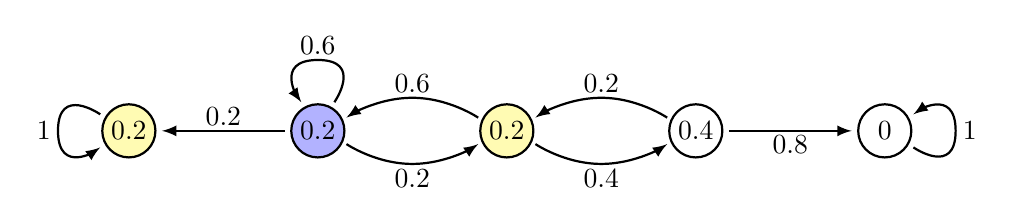
\begin{tikzpicture}[scale=0.6,font=\normalsize,baseline,thick]
            \foreach \x/\xcolor in {1/yellow!30,2/blue!30,3/yellow!30,4/white,5/white} {
                \filldraw[color=black,fill=\xcolor,thick] (4*\x,0) circle (16pt);
            }
            \foreach \x/\xtext in {1/0.2,2/0.2,3/0.2,4/0.4,5/0} {
                \node at (4*\x,0) {\xtext};
            }
            \draw [->,>=latex] plot [smooth,tension=5] coordinates {(8+0.5*0.7,0.866*0.7) (8+0,1.5) (8-0.5*0.7,0.866*0.7)};
            \node at (8,1.8) {0.6};
            \foreach \x in {3,...,4} {
                \draw [->,>=latex] plot [smooth,tension=1] coordinates {(4*\x-0.866*0.7,0.4*0.7) (4*\x-2,0.7) (4*\x-4+0.866*0.7,0.4*0.7)};
            }
            \foreach \x in {2,...,3} {
                \draw [->,>=latex] plot [smooth,tension=1] coordinates {(4*\x+0.866*0.7,-0.4*0.7) (4*\x+2,-0.7) (4*\x+4-0.866*0.7,-0.4*0.7)};
            }
            \draw[->,>=latex] (8-0.7,0) -- (4+0.7,0);
            \draw[->,>=latex] (16+0.7,0) -- (20-0.7,0);
            \node at (6,0.3) {0.2};
            \node at (10,1) {0.6};
            \node at (14,1) {0.2};
            \node at (10,-1) {0.2};
            \node at (14,-1) {0.4};
            \node at (18,-0.3) {0.8};
            \draw [->,>=latex] plot [smooth,tension=5] coordinates {(4-0.866*0.7,0.5*0.7) (4-1.5,0) (4-0.866*0.7,-0.5*0.7)};
            \node at (2.2,0) {1};
            \draw [->,>=latex] plot [smooth,tension=5] coordinates {(20+0.866*0.7,-0.5*0.7) (20+1.5,0) (20+0.866*0.7,0.5*0.7)};
            \node at (21.8,0) {1};
        \end{tikzpicture}
        % \caption{$\mathbf{h}$ after firing to $v_2$, shown in blue.
        % States with updated hungers are shown in yellow.}
        % \label{subfig:ex1fire1}
    \end{subfigure}
    
    \vspace{-0.5mm}
    
    \begin{subfigure}{\textwidth}
        \centering
        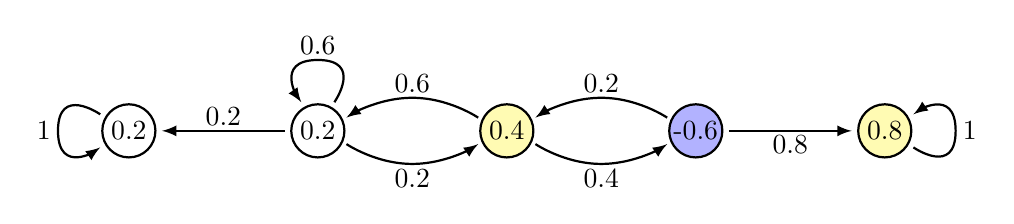
\begin{tikzpicture}[scale=0.6,font=\normalsize,baseline,thick]
            \foreach \x/\xcolor in {1/white,2/white,3/yellow!30,4/blue!30,5/yellow!30} {
                \filldraw[color=black,fill=\xcolor,thick] (4*\x,0) circle (16pt);
            }
            \foreach \x/\xtext in {1/0.2,2/0.2,3/0.4,4/-0.6,5/0.8} {
                \node at (4*\x,0) {\xtext};
            }
            \draw [->,>=latex] plot [smooth,tension=5] coordinates {(8+0.5*0.7,0.866*0.7) (8+0,1.5) (8-0.5*0.7,0.866*0.7)};
            \node at (8,1.8) {0.6};
            \foreach \x in {3,...,4} {
                \draw [->,>=latex] plot [smooth,tension=1] coordinates {(4*\x-0.866*0.7,0.4*0.7) (4*\x-2,0.7) (4*\x-4+0.866*0.7,0.4*0.7)};
            }
            \foreach \x in {2,...,3} {
                \draw [->,>=latex] plot [smooth,tension=1] coordinates {(4*\x+0.866*0.7,-0.4*0.7) (4*\x+2,-0.7) (4*\x+4-0.866*0.7,-0.4*0.7)};
            }
            \draw[->,>=latex] (8-0.7,0) -- (4+0.7,0);
            \draw[->,>=latex] (16+0.7,0) -- (20-0.7,0);
            \node at (6,0.3) {0.2};
            \node at (10,1) {0.6};
            \node at (14,1) {0.2};
            \node at (10,-1) {0.2};
            \node at (14,-1) {0.4};
            \node at (18,-0.3) {0.8};
            \draw [->,>=latex] plot [smooth,tension=5] coordinates {(4-0.866*0.7,0.5*0.7) (4-1.5,0) (4-0.866*0.7,-0.5*0.7)};
            \node at (2.2,0) {1};
            \draw [->,>=latex] plot [smooth,tension=5] coordinates {(20+0.866*0.7,-0.5*0.7) (20+1.5,0) (20+0.866*0.7,0.5*0.7)};
            \node at (21.8,0) {1};
        \end{tikzpicture}
        % \caption{$\mathbf{h}$ after firing to $v_4$, shown in blue.
        % States with updated hungers are shown in yellow.}
        % \label{subfig:ex1fire2}
    \end{subfigure}
    
    \vspace{-0.5mm}
    
    \begin{subfigure}{\textwidth}
        \centering
        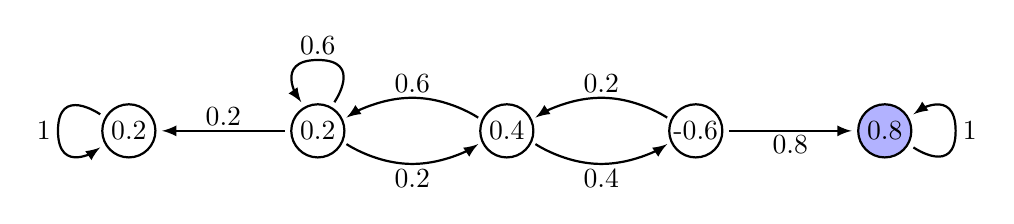
\begin{tikzpicture}[scale=0.6,font=\normalsize,baseline,thick]
            \foreach \x/\xcolor in {1/white,2/white,3/white,4/white,5/blue!30} {
                \filldraw[color=black,fill=\xcolor,thick] (4*\x,0) circle (16pt);
            }
            \foreach \x/\xtext in {1/0.2,2/0.2,3/0.4,4/-0.6,5/0.8} {
                \node at (4*\x,0) {\xtext};
            }
            \draw [->,>=latex] plot [smooth,tension=5] coordinates {(8+0.5*0.7,0.866*0.7) (8+0,1.5) (8-0.5*0.7,0.866*0.7)};
            \node at (8,1.8) {0.6};
            \foreach \x in {3,...,4} {
                \draw [->,>=latex] plot [smooth,tension=1] coordinates {(4*\x-0.866*0.7,0.4*0.7) (4*\x-2,0.7) (4*\x-4+0.866*0.7,0.4*0.7)};
            }
            \foreach \x in {2,...,3} {
                \draw [->,>=latex] plot [smooth,tension=1] coordinates {(4*\x+0.866*0.7,-0.4*0.7) (4*\x+2,-0.7) (4*\x+4-0.866*0.7,-0.4*0.7)};
            }
            \draw[->,>=latex] (8-0.7,0) -- (4+0.7,0);
            \draw[->,>=latex] (16+0.7,0) -- (20-0.7,0);
            \node at (6,0.3) {0.2};
            \node at (10,1) {0.6};
            \node at (14,1) {0.2};
            \node at (10,-1) {0.2};
            \node at (14,-1) {0.4};
            \node at (18,-0.3) {0.8};
            \draw [->,>=latex] plot [smooth,tension=5] coordinates {(4-0.866*0.7,0.5*0.7) (4-1.5,0) (4-0.866*0.7,-0.5*0.7)};
            \node at (2.2,0) {1};
            \draw [->,>=latex] plot [smooth,tension=5] coordinates {(20+0.866*0.7,-0.5*0.7) (20+1.5,0) (20+0.866*0.7,0.5*0.7)};
            \node at (21.8,0) {1};
        \end{tikzpicture}
        \caption{$\mathbf{h}$ as the chip fires successively to $v_2$, $v_4$, and $v_5$, shown in blue. Updated hungers are shown in yellow.}
        \label{subfig:ex1fire3}
    \end{subfigure}
    \begin{subfigure}{\textwidth}
        \centering
        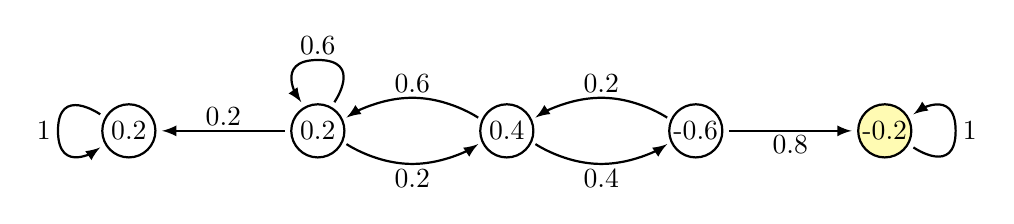
\begin{tikzpicture}[scale=0.6,font=\normalsize,baseline,thick]
            \foreach \x/\xcolor in {1/white,2/white,3/white,4/white,5/yellow!30} {
                \filldraw[color=black,fill=\xcolor,thick] (4*\x,0) circle (16pt);
            }
            \foreach \x/\xtext in {1/0.2,2/0.2,3/0.4,4/-0.6,5/-0.2} {
                \node at (4*\x,0) {\xtext};
            }
            \draw [->,>=latex] plot [smooth,tension=5] coordinates {(8+0.5*0.7,0.866*0.7) (8+0,1.5) (8-0.5*0.7,0.866*0.7)};
            \node at (8,1.8) {0.6};
            \foreach \x in {3,...,4} {
                \draw [->,>=latex] plot [smooth,tension=1] coordinates {(4*\x-0.866*0.7,0.4*0.7) (4*\x-2,0.7) (4*\x-4+0.866*0.7,0.4*0.7)};
            }
            \foreach \x in {2,...,3} {
                \draw [->,>=latex] plot [smooth,tension=1] coordinates {(4*\x+0.866*0.7,-0.4*0.7) (4*\x+2,-0.7) (4*\x+4-0.866*0.7,-0.4*0.7)};
            }
            \draw[->,>=latex] (8-0.7,0) -- (4+0.7,0);
            \draw[->,>=latex] (16+0.7,0) -- (20-0.7,0);
            \node at (6,0.3) {0.2};
            \node at (10,1) {0.6};
            \node at (14,1) {0.2};
            \node at (10,-1) {0.2};
            \node at (14,-1) {0.4};
            \node at (18,-0.3) {0.8};
            \draw [->,>=latex] plot [smooth,tension=5] coordinates {(4-0.866*0.7,0.5*0.7) (4-1.5,0) (4-0.866*0.7,-0.5*0.7)};
            \node at (2.2,0) {1};
            \draw [->,>=latex] plot [smooth,tension=5] coordinates {(20+0.866*0.7,-0.5*0.7) (20+1.5,0) (20+0.866*0.7,0.5*0.7)};
            \node at (21.8,0) {1};
        \end{tikzpicture}
        \caption{$\mathbf{h}$ after removing chip from $v_5$, shown in yellow.}
        \label{subfig:ex1remove}
    \end{subfigure}
    \caption{The hunger game on $G$ from \cref{fig:ex1G} after inserting a chip at $v_3$.}
    \label{fig:ex1H}
\end{figure}

Notice that the total hunger is 0 at the start,
increases to 1 when the chip is added at $v_3$,
stays 1 as the chip moves through $G$,
and decreases to 0 when the chip is removed at the end.

\end{example}

Since increasing the hunger at every vertex by the same amount
has no effect on the dynamics of the hunger game,
when our Markov chain is finite we will often assume 
that total hunger is 0.
% Do we do this? Do we need to?
